\documentclass[12pt]{article}
% Required Packages
\usepackage[utf8]{inputenc}
\usepackage{geometry}
\geometry{letterpaper, margin=1in}
\usepackage{subcaption}
\usepackage{amsmath}
\usepackage{graphicx}
\usepackage{booktabs}
\usepackage[numbers,super]{natbib} % For ACS citation style baseline
\usepackage{hyperref}
\usepackage{fontawesome5} % for using icons
\usepackage[dvipsnames]{xcolor}
\usepackage{textcomp}
\usepackage{pdfpages}

\begin{document}

\begin{center}
    \Large \textbf{Lab \#2: Silver Equilibrium}
\end{center}
\vspace{0.5em}

\begin{minipage}[t]{0.5\textwidth}
    \small
    \textbf{Name:} Yuchen Shi \\
    \textbf{Lab Partner:} Yizhe Dai, Siqi Li \\ 
    \textbf{Section:} 001
\end{minipage}%
\begin{minipage}[t]{0.5\textwidth}
    \small \raggedleft
    \textbf{Date Performed:} 2026-02-24 \\ 
    \textbf{Date Submitted:} 2026-03-10 
\end{minipage}
\vspace{1.5em}

\begin{abstract}
In this experiment, the equilibrium of silver ion with chloride ion, iodide, and ammonia were studied by monitoring the time dependent electric potential curve of a electrochemical cell with Cu and Ag as electrodes. $1.00\times10^{-4}$ M AgNO$_3$ solution was used to determine the cell constant. With potential stabilized, NH$_4$Cl, three portions of NH$_3$, and KI solution were added to determine silver concentrations and the Nernst equation. Debye-Huckel corrections were used to obtain solubility products for AgCl and AgI. A linear fit of $\log([\mathrm{Ag(NH_3)_p^+}]/[\mathrm{Ag^+}])$ versus $\log[NH_3]$ was used to estimate the coordination number and formation constant of the silver-ammonia complex. The calculated properties from experimental data were $K_{sp}(\mathrm{AgCl})=(1.375\pm0.1050)\times10^{-10}$ with an error rate of 22.32 \% , $K_{sp}(\mathrm{AgI})=(6.872\pm0.2277)\times10^{-17}$ with an error rate of 19.34 \% , and $K_f=(3.956\pm0.4929)\times10^{7}$ with 95\% confidence and an error rate of 147.3 \% . The linear regression confirmed $p=2.104\pm0.04850$, indicating that the dominant complex was [Ag(NH$_3$)$_2$]$^+$.
\end{abstract}


\section*{Introduction}
In a multi-component solution, different species of ions interact complicatedly with many physical and chemical processes happening, such as coordination, precipitation, etc. Determination of related property constants can help us predict the their chemical behavior and rationally design reactions.

The purpose of this experiment was to determine the equilibrium behavior of silver ions with three ligands, Cl$^-$, I$^-$, and NH$_3$ by measuring the time-dependent electric potential in a electrochemical cell. A silver and a copper electrodes are used to monitor changes in Ag$^+$ activity during a sequence of ligand additions.The observed potentials can be converted into free Ag$^+$ concentrations using the Nernst equation. \cite{lab_manual}
\begin{equation}
E_{\mathrm{obs}} = C + 0.0592\log_{10}[\mathrm{Ag^+}]
\label{eq:nernst}
\end{equation}
assuming the temperature is $25 ^oC$. Once $C$ is obtained from a solution of known silver concentration, later equilibrated electric potential can be used to compute $[\mathrm{Ag^+}]$. The silver ion concentrations can then be used to evaluate the solubility products of AgCl and AgI, the stoichiometry, and formation constant of the silver-ammonia complex.

Assume ideal conditions, the measured concentrations were used to evaluate\cite{lab_manual}
\begin{equation}
Q_{sp}(AgX)=[\mathrm{Ag^+}][\mathrm{X^-}], \qquad K_{sp}(AgX)=\gamma_{\pm}^{2}Q_{sp}
\end{equation}
with $\mathrm{X^-}=\mathrm{Cl^-}$ or $\mathrm{I^-}$. The activity coefficient $\gamma_{\pm}$ can be estimated from the Debye-Huckel law from\cite{lab_manual}
\begin{equation}
\log\gamma_{\pm}=-|z_+z_-|AI^{\frac{1}{2}}
\end{equation}
where $z$ is the number charges of ions in the compound and the ionic strength $I$ is defined as $\frac{1}{2}\sum_iz_i^2m_i$.

For the ammonia complex, the formation constant is\cite{lab_manual}
\begin{equation}
K_f = \frac{[\mathrm{Ag(NH_3)_p^+}]}{[\mathrm{Ag^+}][\mathrm{NH_3}]^{p}}.
\end{equation}
Assuming that essentially all dissolved silver is present as complex and that binding consumes a negligible fraction of the large excess of NH$_3$, the data can be rearranged into the linear form\cite{lab_manual}
\begin{equation}
Y = \log\left(\frac{[\mathrm{Ag(NH_3)_p^+}]}{[\mathrm{Ag^+}]}\right)=\log K_f+p\log[\mathrm{NH_3}],
\label{eq:fit}
\end{equation}
so that the slope gives the coordination number $p$ and the intercept gives $\log K_f$. The properties of the ammonia complex can be computed and analyzed then. 



\section*{Experimental}
The experiment was carried out with a silver electrode and a copper electrode connected to a Logger Pro voltage interface. The voltage interface was calibrated with 1.5V dry cell and voltmeter before doing the experiment. Both electrolytes were placed in a glass electrochemical vessel. The silver electrode was first cleaned by immersion into hot sodium bicarbonate solution with aluminum foil before use. The copper electrode was placed in 0.1 M CuSO$_4$ solution, closely above a salt bridge prepared in advance. 10.00 mL of standardized 0.0010 M AgNO$_3$ and 0.010 M NH$_4$NO$_3$ was diluted to 100.0 mL using volumetric flask, and transferred to the electrochemical cell. Magnetic stir was used to equilibrate the solution during the whole experiment and get a stable baseline potential to get start with.

Voltage was then recorded every two seconds for a total length of 3000 seconds. First, 10.00 mL of 0.0010 M NH$_4$Cl was added to precipitate AgCl. Light white precipitation was observed shortly after adding the solution. After the potential stabilized, 10.00 mL mixture of 2.0 M NH$_3$ containing 0.010 M NH$_4$NO$_3$ were added three times, each followed by equilibration to a new potential plateau in around five minutes. Finally, 10.00 mL of 0.010 M KI was added and the final stabilized potential was recorded till the end. The solution became dark green first and turned milky afterwards. The potential-time curve was then analyzed in Logger Pro and their mean voltages and standard deviations were obtained.

The linear regression for Ag-NH$_3$ complex was plotted using Numpy\cite{harris2020array}, Matplotlib\cite{Hunter2007}, and Pandas\cite{reback2020pandas} libraries in Python. The linear regression parameters were determined by SciPy\cite{2020SciPy} library automatically. 

\section*{Results}
Figure 1 shows the potential-time curve with linear regressions done by Logger Pro. Six stable plateaus were identified and analyzed to obtain the silver concentrations at each stage. The mean potential and standard deviation of each plateau are collected in Table 1.

\begin{figure}[htb!]
    \centering
    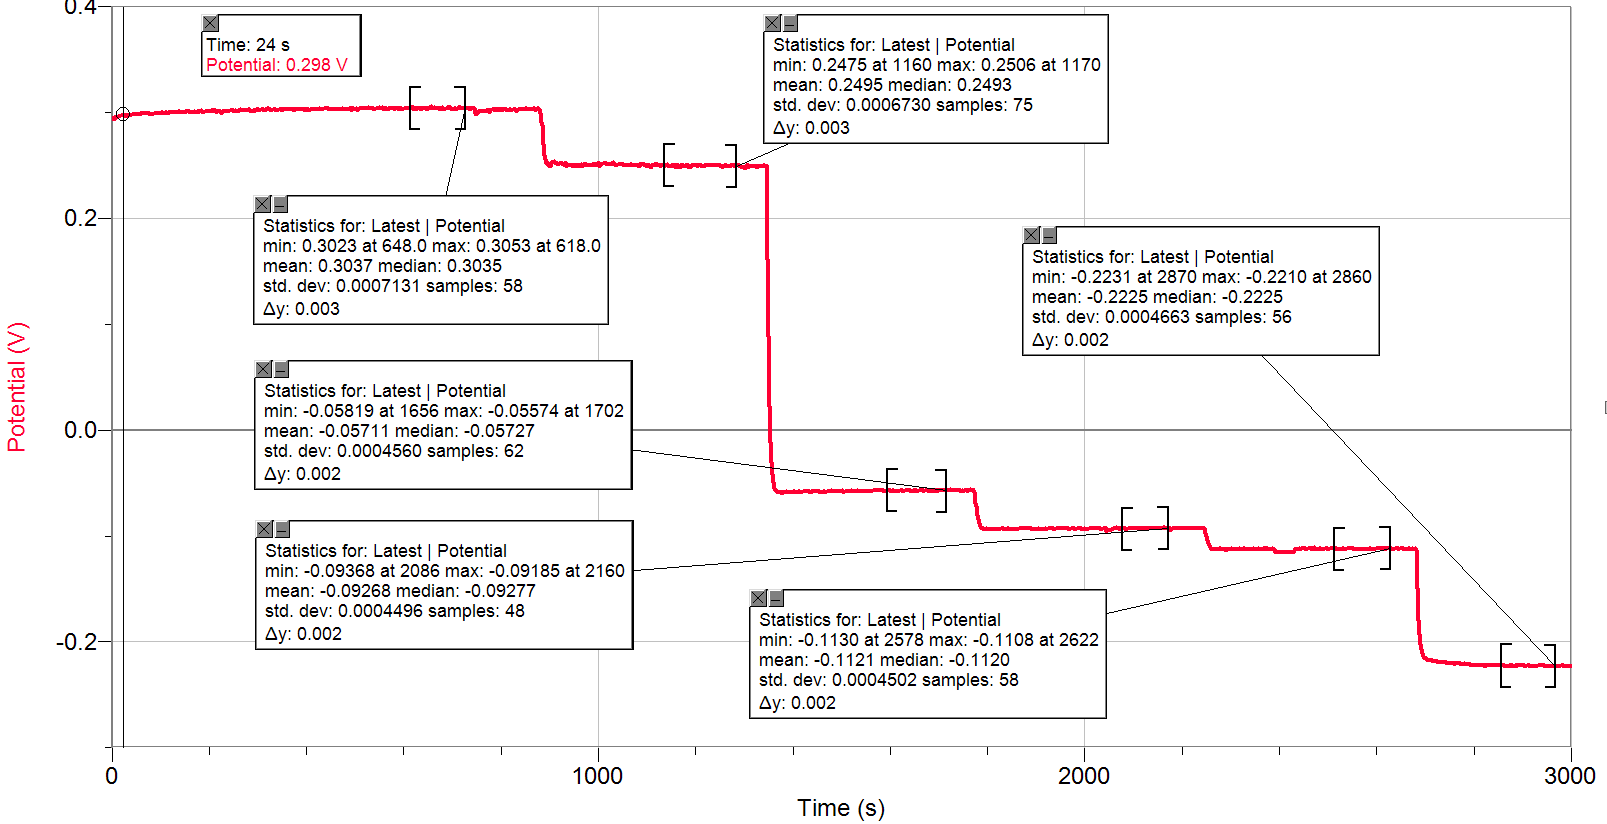
\includegraphics[width=1\textwidth]{voltage_time_plot.png}
    \caption{Voltage as a function of time during sequential addition of NH$_4$Cl, three aliquots of NH$_3$, and KI. The highlighted plateaus were used to calculate average stabilized potentials and their standard deviations.}
    \label{fig:trace}
\end{figure}

\begin{table}[htb!]
\centering
\caption{Stabilized cell potentials read from the processed Logger Pro trace.}
\label{tab:plateaus}
\begin{tabular}{lll}
\toprule
Stage & $E_{\mathrm{obs}}$ / V & Standard deviation / V \\
\midrule
Initial AgNO$_3$ solution ($E_1$) & 0.3037 & 0.0007131 \\
After NH$_4$Cl addition ($E_2$) & 0.2495 & 0.0006730 \\
After 10 mL NH$_3$ ($E_3$) & $-0.05711$ & 0.0004560 \\
After 20 mL NH$_3$ ($E_4$) & $-0.09268$ & 0.0004496 \\
After 30 mL NH$_3$ ($E_5$) & $-0.1121$ & 0.0004502 \\
After KI addition ($E_6$) & $-0.2225$ & 0.0004663 \\
\bottomrule
\end{tabular}
\end{table}

\subsection*{Nerst Constant}
Using Eq.1 and $[\mathrm{Ag^+}]=1.00\times 10^{-4}{M}$ for the initial solution,
\begin{equation}
C=E_0-0.0592\log(1.00\times10^{-4})=0.5405\pm0.0007131\ \mathrm{V}.
\end{equation}
where the uncertainty in $C$ was taken directly as the standard deviation of the potential with initial Ag$^+$ concentration was treated as exact.

\subsection*{AgCl Equilibrium}
After addition of NH$_4$Cl, the silver concentration was obtained from Eq.1
\begin{equation}
[\mathrm{Ag^+}]_{\mathrm{AgCl}} = 10^{(E_{\mathrm{AgCl}}-C)/0.0592} = (1.2147\pm0.0463)\times10^{-5}\ \mathrm{M}.
\end{equation}
As the initial Ag$^+$ and Cl$^-$ concentrations were equal before precipitation, we can assume that $[\mathrm{Ag^+}]=[\mathrm{Cl^-}]$, giving
\begin{equation}
Q_{sp}(\mathrm{AgCl})=[\mathrm{Ag^+}]^2=(1.475\pm0.113)\times10^{-10}.
\end{equation}
After dilution to 110 mL, the concentration of NH$_4$NO$_3$ was $9.09\times10^{-4}$ M, so $I=9.09\times10^{-4}$ and $\gamma_{\pm}=0.9653$. Therefore,
\begin{equation}
K_{sp}(\mathrm{AgCl})=\gamma_{\pm}^{2}Q_{sp}=(1.375\pm0.1050)\times10^{-10}.
\end{equation}


\subsection*{Silver-ammonia Complex}
The silver concentrations after the three ammonia additions can be calculated as
\begin{align}
[\mathrm{Ag^+}]_{E_3} &= (8.04\pm0.26)\times10^{-11}\ \mathrm{M} \\
[\mathrm{Ag^+}]_{E_4} &= (2.016\pm0.066)\times10^{-11}\ \mathrm{M} \\
[\mathrm{Ag^+}]_{E_5} &= (9.47\pm0.31)\times10^{-12}\ \mathrm{M}.
\end{align}
The concentrations of $NH_3$ and $Ag(NH_3)_p^+$ in diluted solution are calculated as
\begin{equation}
[\mathrm{Ag(NH_3)_p^+}] = (1.000\times10^{-4})\frac{100}{110+V}
\end{equation}
and
\begin{equation}
[\mathrm{NH_3}] = \frac{V(2.00)}{110+V},
\end{equation}
values of $Y$ and $\log[NH_3]$ were calculated for $V=10$, 20, and 30 mL. 

Linear regression of Eq.5 show that
\begin{equation}
Y=(2.104\pm0.04850)\log[NH_3]+(7.655\pm0.02805), \qquad R^2=0.9999.
\end{equation}
The regression is shown in Figure 2. The slope corresponds to $p=2.104\pm0.04850$, which rounds to $p=2$.

\begin{figure}[htb!]
    \centering
    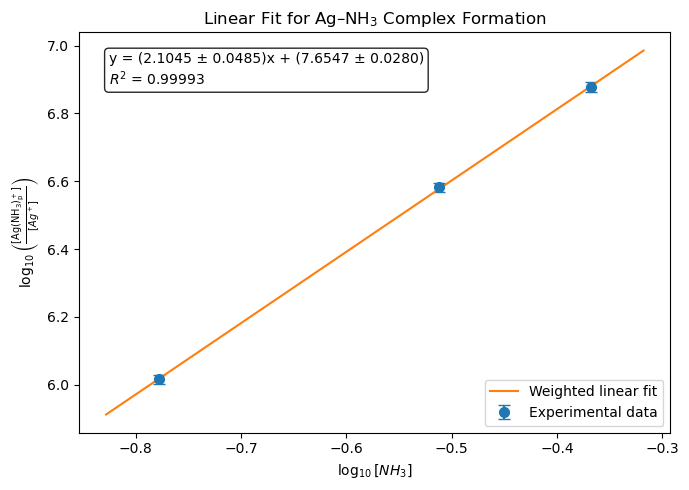
\includegraphics[width=1\textwidth]{linear_regression.png}
    \caption{Linear regression of $Y=\log([\mathrm{Ag(NH_3)_p^+}]/[\mathrm{Ag^+}])$ versus $\log[NH_3]$. The displayed fit reports the slope ($p = 2.10 \pm 0.05$) and intercept ($b = 7.65 \pm 0.03$), with $R^2 = 0.9999$.}
    \label{fig:fit}
\end{figure}

As $logK_f=b$, from the intercept, the graph-based formation constant is
\begin{equation}
K_{f,\mathrm{graph}} = 10^{7.655}=(4.515\pm0.2911)\times10^{7}.
\end{equation}
Using the rounded integer value $p=2$, the formation constants are calculated from the three individual points
\begin{align}
K_{f,1}&=3.732\times10^{7} \\
K_{f,2}&=4.031\times10^{7} \\
K_{f,3}&=4.107\times10^{7}.
\end{align}
With averaging, error propagation and analysis, we can have
\begin{equation}
\bar K_f = 3.956\times10^{7}, \qquad S_{K_f}=1.984\times10^{6}.
\end{equation}
Using $t=4.303$ for $n=3$ at 95\% confidence,
\begin{equation}
\lambda_{K_f}=t\frac{S_{K_f}}{\sqrt{n}}=4.93\times10^{6},
\end{equation}
so the final pointwise estimate is
\begin{equation}
K_f=(3.956\pm0.4929)\times10^{7}
\end{equation}
with 95\% confidence.

\subsection*{AgI equilibrium}
The final stabilized electric potential gives that
\begin{equation}
[\mathrm{Ag^+}]_{\mathrm{AgI}}=(1.293\pm0.043)\times10^{-13}\ \mathrm{M}.
\end{equation}
As suggested in the guideline, because KI was added in largely excess relative to the initial silver concentration, the iodide concentration could not be approximated as equal to the silver concentration. Instead, the remaining iodide was calculated from the initial moles of iodide minus the moles required to precipitate the initial silver concentrations.
\begin{equation}
[\mathrm{I^-}]_{\mathrm{left}}=6.00\times10^{-4}\ \mathrm{M}.
\end{equation}
Thus,
\begin{equation}
Q_{sp}(\mathrm{AgI})=[\mathrm{Ag^+}][\mathrm{I^-}]_{\mathrm{left}}=(7.756\pm0.2570)\times10^{-17}.
\end{equation}
At this stage the NH$_4$NO$_3$ concentration was 2.667$10^{-3}$ M, given $\gamma_{\pm}=0.9413$.
\begin{equation}
K_{sp}(\mathrm{AgI})=\gamma_{\pm}^{2}Q_{sp}=(6.872\pm0.2277)\times10^{-17}.
\end{equation}

The final numerical results are summarized in Table 2.

\begin{table}[htb!]
\centering
\caption{Summary of calculated equilibrium constants. Literature values for $K_{sp}$ were taken from the CRC Handbook\cite{lide2002handbook}, and the literature value for $K_f$ was taken from the LibreTexts table\cite{lit_constants} of complex-ion formation constants.}
\label{tab:final}
\begin{tabular}{llll}
\toprule
Quantity & Experimental value & Literature value & Error Rate\\
\midrule
$K_{sp}(\mathrm{AgCl})$ & $(1.375\pm0.1050)\times10^{-10}$ & $1.77\times10^{-10}$  & 22.32 \%\\
$K_{sp}(\mathrm{AgI})$ & $(6.872\pm0.2277)\times10^{-17}$ & $8.52\times10^{-17}$  & 19.34 \%\\
$K_f$ from graph & $(4.515\pm0.2911)\times10^{7}$ & $1.6\times10^{7}$  & 182.2 \%\\
Averaged $K_f$ & $(3.956\pm0.4929)\times10^{7}$ & $1.6\times10^{7}$  & 147.3 \% \\
\bottomrule
\end{tabular}
\end{table}

\section*{Discussion}
In general, the electrochemical method basically described three distinct kinds of silver equilibrium with voltage-time curve. The AgCl and AgI plateaus were well separated from the baseline potential, and the ammonia additions gradually decreased the free silver concentration. The linearity of the $Y$-$\log[NH_3]$ plot was great ($R^2=0.9999$), and the fitted slope $p=2.104\pm0.04850$ shows that the dominant dissolved complex was [Ag(NH$_3$)$_2$]$^+$. This conclusion is chemically reasonable because silver(I) ion commonly forms a linear diammine complex in aqueous ammonia solutions.

The measured $K_{sp}(\mathrm{AgCl})$ was lower than the literature value by 22.32\%, while $K_{sp}(\mathrm{AgI})$ was lower by 19.34\%. These two deviations are similar in magnitude and direction, which suggests the presence of a common systematic contribution. The most likely source is the use of $25 ^oC$ in the Nernst slope rather than the actual measured temperature. A small temperature mismatch affects all converted Ag$^+$ concentrations in the same direction and introduce errors in related properties. Another systematic error could arise from the assumption that NH$_4$NO$_3$ alone determines the ionic strength for both salts. Although this approximation largely simplifies calculations, it neglects small contributions from the reacting ions themselves.

The formation constant showed a larger discrepancy from the literature value, where the graph-based value is higher the literature value by 182\%, and the averaged value is higher by 147.3\%. It's shown that the pointwise averaging method is more accurate. The complex-formation calculation is particularly sensitive because $[\mathrm{Ag^+}]$ after ammonia addition is extremely small. So, a small uncertainty in electric potential can propagate into a large fractional uncertainty in $K_f$. In addition, the intercept method determines $K_f$ by extrapolating the regression to $\log[NH_3]=0$, which lies outside the narrow range of measured ammonia concentrations. Also, the initial calibration of the Logger Pro voltmeter could also systematically alter the results, resonating with other errors in $K_{sp}$.

Overall, the experiment demonstrated that emf measurements can be used to determine silver equilibrium constants in dilute solution. The main conclusions are that the dominant ammonia complex was [Ag(NH$_3$)$_2$]$^+$, the measured solubility products were of the correct order of magnitude but somewhat lower than literature values, and the formation constant obtained from the present dataset was systematically higher than the accepted value. These errors can be further corrected by improving experimental procedures and apparatus. 



\section*{Conclusion}

The potential measurements obtained with the silver electrode were used to determine the solubility products of AgCl and AgI and to analyze the formation of the silver-ammonia complex. From the AgCl portion of the experiment, the activity-corrected solubility product was found to be \(K_{sp}(\mathrm{AgCl})=(1.375 \pm 0.1050)\times10^{-10}\). From the AgI portion, the corrected value was \(K_{sp}(\mathrm{AgI})=(6.872  \pm 0.2277)\times10^{-17}\). Linear regression of \(\log([\mathrm{Ag(NH_3)_p^+}]/[Ag^+])\)-\(\log[NH_3]\) gave \(p=2.104\pm0.04850\), indicating that the dominant complex was \([\mathrm{Ag(NH_3)_2}]^+\). The corresponding $K_f$ were calculated to be $4.515 \pm 0.2911\times10^{7}$ directly from the graph and $3.956 \pm 0.4929\times10^{7}$ from averaging points.

Overall, the experiment verified the Nernst equation and activity corrections in equilibrium analysis. The experimental constants deviated from literature values, likely due to voltameter calibration and the approximations used in calculations.


\newpage
% References section 
% Must follow American Chemical Society (ACS) format. 
\bibliographystyle{achemso} % Uses the ACS formatting style
\bibliography{references} % Ensure you create a references.bib file in your directory

\newpage
\section*{Appendix}
\addcontentsline{toc}{section}{Appendix}
% Include supplementary material (raw output, sample calculations) 
The raw data and corresponding analysis script are available on \href{https://github.com/EasonShi0624/26Spring-PChemLab/tree/main/Lab_2_Silver_Equilibrium}{\textcolor{RoyalBlue}{GitHub} \faGithub}

\begin{figure}[htbp]
    \centering
    
\includegraphics[width=0.7\linewidth, keepaspectratio, page=1]{Lab Computation.pdf}
    \caption{Computations of Values and Error Analysis (Page 1)}
    \label{fig:lab_comp_p1}
\end{figure}

\begin{figure}[htbp]
    \centering
    
\includegraphics[width=0.9\linewidth, keepaspectratio, page=2]{Lab Computation.pdf}
    \caption{Computations of Values and Error Analysis (Page 2)}
    \label{fig:lab_comp_p1}
\end{figure}


\begin{figure}[htbp]
    \centering
    
\includegraphics[width=0.9\linewidth, keepaspectratio, page=3]{Lab Computation.pdf}
    \caption{Computations of Values and Error Analysis (Page 3)}
    \label{fig:lab_comp_p1}
\end{figure}


\begin{figure}[htbp]
    \centering
    
\includegraphics[width=0.9\linewidth, keepaspectratio, page=4]{Lab Computation.pdf}
    \caption{Computations of Values and Error Analysis (Page 4)}
    \label{fig:lab_comp_p1}
\end{figure}


\begin{figure}[htbp]
    \centering
    
\includegraphics[width=0.9\linewidth, keepaspectratio, page=5]{Lab Computation.pdf}
    \caption{Computations of Values and Error Analysis (Page 5)}
    \label{fig:lab_comp_p1}
\end{figure}

\begin{figure}[htbp]
    \centering
    
\includegraphics[width=0.9\linewidth, keepaspectratio, page=6]{Lab Computation.pdf}
    \caption{Computations of Values and Error Analysis (Page 6)}
    \label{fig:lab_comp_p1}
\end{figure}


\begin{figure}[htbp]
    \centering
    
\includegraphics[width=0.9\linewidth, keepaspectratio, page=7]{Lab Computation.pdf}
    \caption{Computations of Values and Error Analysis (Page 7)}
    \label{fig:lab_comp_p1}
\end{figure}


\begin{figure}[htbp]
    \centering
    
\includegraphics[width=0.9\linewidth, keepaspectratio, page=8]{Lab Computation.pdf}
    \caption{Computations of Values and Error Analysis (Page 8)}
    \label{fig:lab_comp_p1}
\end{figure}





\begin{figure}[htbp]
    \centering
    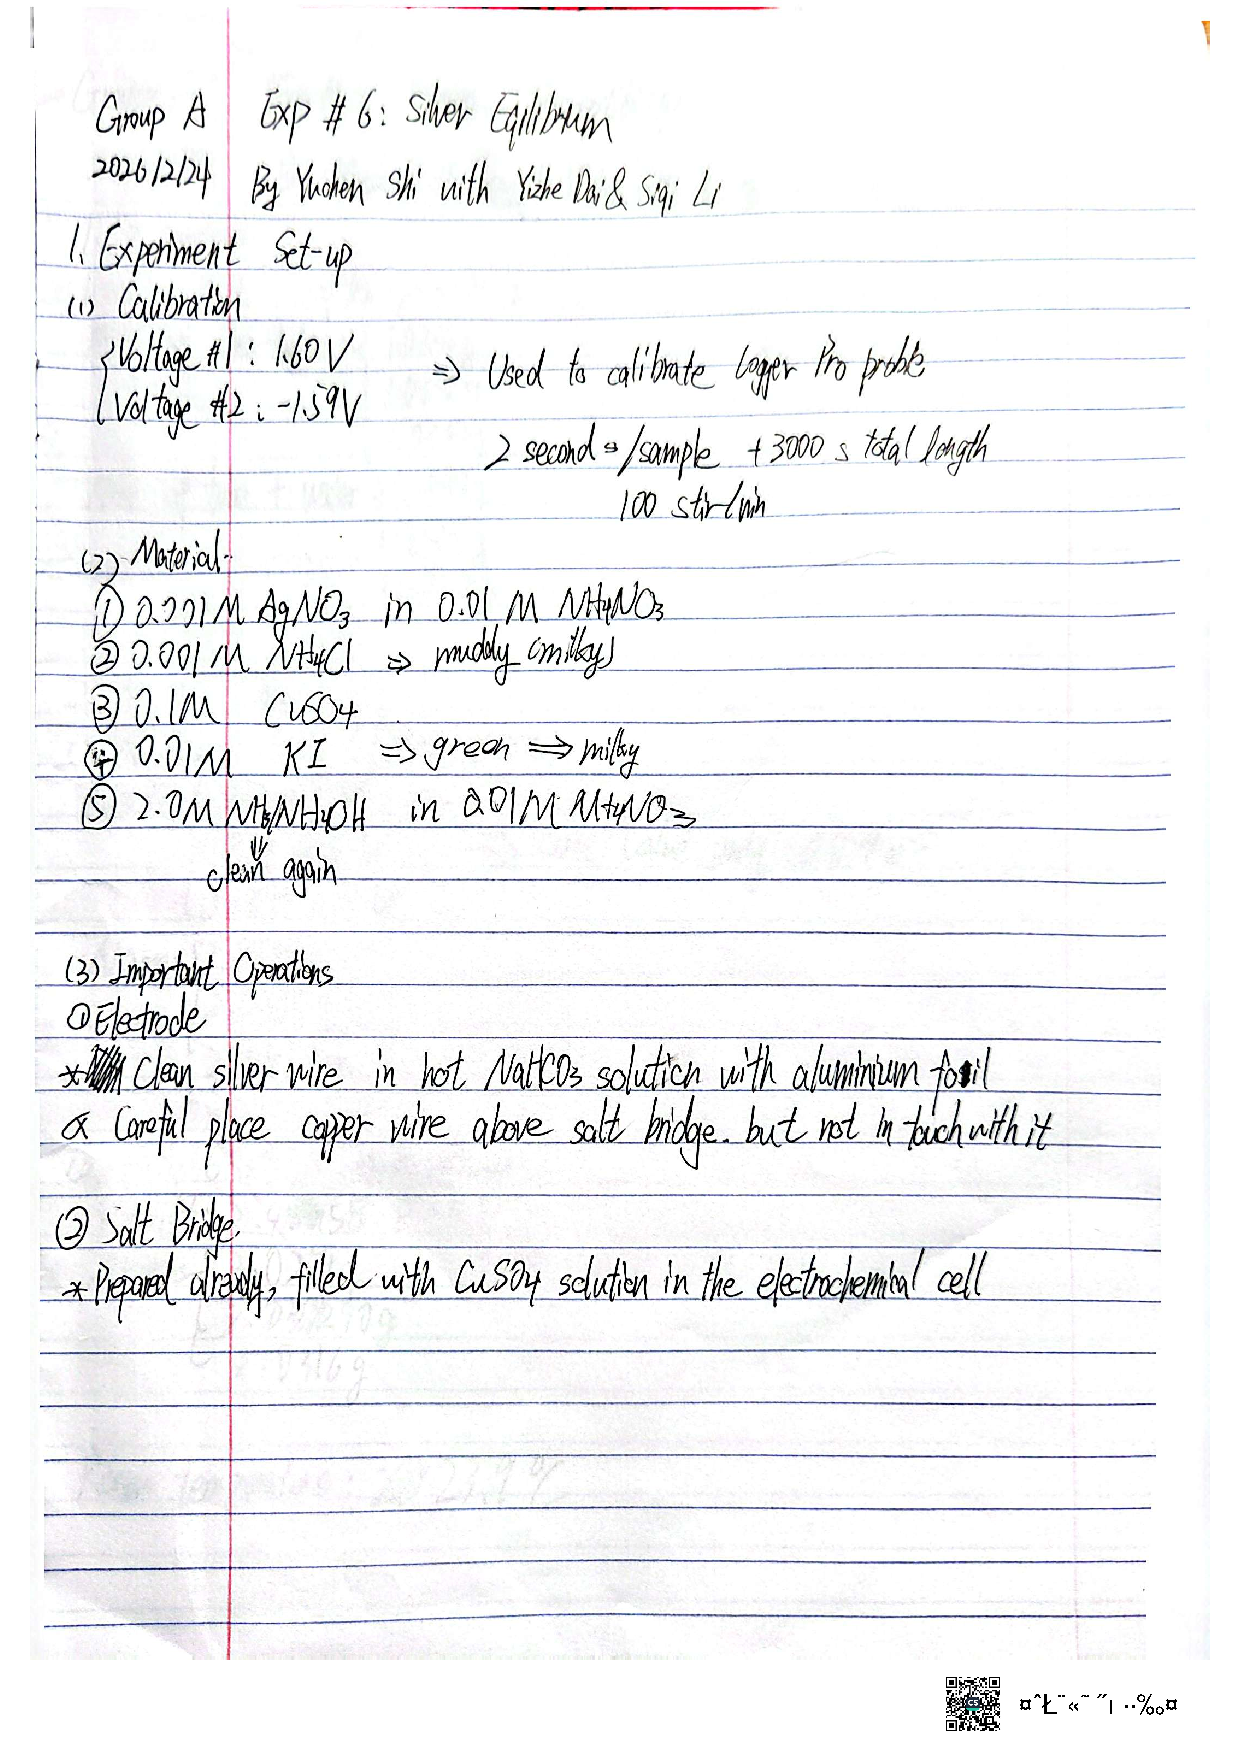
\includegraphics[width=0.9\linewidth, keepaspectratio, page=1]{labnotes2.pdf}
    \caption{Raw Lab Notes}
    \label{fig:lab_notes}
\end{figure}


\end{document}